{\begingroup%
  \makeatletter%
  \providecommand\color[2][]{%
    \errmessage{(Inkscape) Color is used for the text in Inkscape, but the package 'color.sty' is not loaded}%
    \renewcommand\color[2][]{}%
  }%
  \providecommand\transparent[1]{%
    \errmessage{(Inkscape) Transparency is used (non-zero) for the text in Inkscape, but the package 'transparent.sty' is not loaded}%
    \renewcommand\transparent[1]{}%
  }%
  \providecommand\rotatebox[2]{#2}%
  \newcommand*\fsize{\dimexpr\f@size pt\relax}%
  \newcommand*\lineheight[1]{\fontsize{\fsize}{#1\fsize}\selectfont}%
  \ifx\svgwidth\undefined%
    \setlength{\unitlength}{538.58267717bp}%
    \ifx\svgscale\undefined%
      \relax%
    \else%
      \setlength{\unitlength}{\unitlength * \real{\svgscale}}%
    \fi%
  \else%
    \setlength{\unitlength}{\svgwidth}%
  \fi%
  \global\let\svgwidth\undefined%
  \global\let\svgscale\undefined%
  \makeatother%
  \begin{picture}(1,0.78947368)%
    \lineheight{1}%
    \setlength\tabcolsep{0pt}%
    \put(0,0){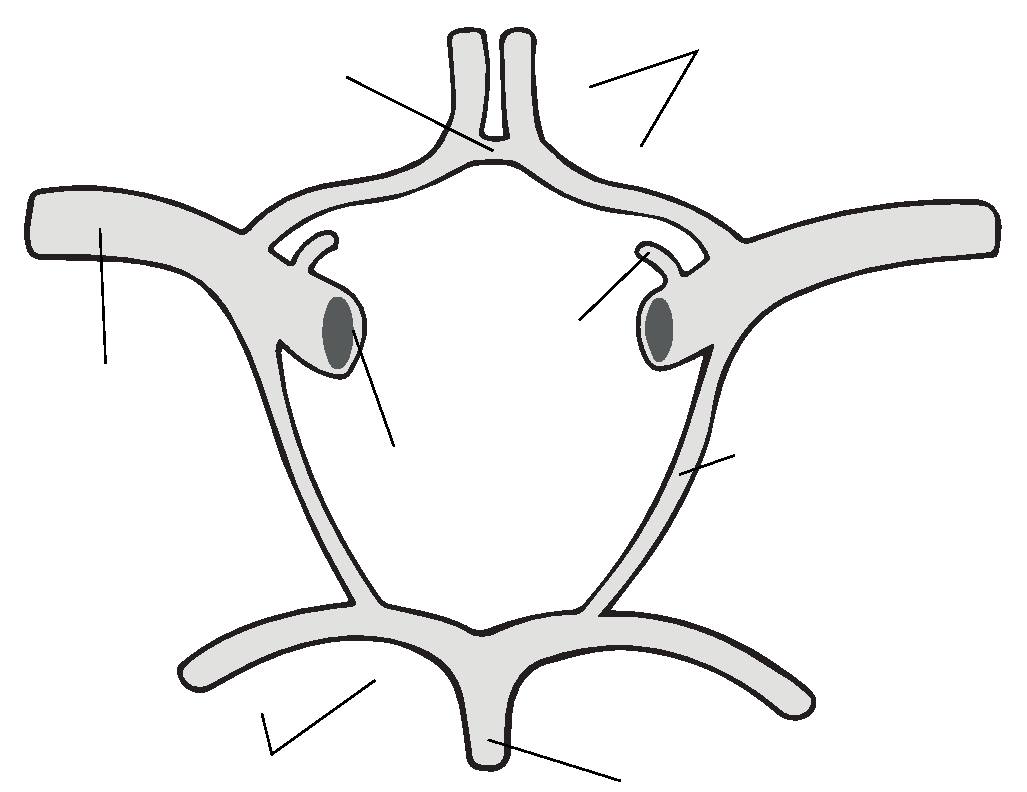
\includegraphics[width=\unitlength]{chapter3/Figures/cow.pdf}}%
    \put(0.01,0.38){\begin{tabular}[t]{l}Middle Cerebral\\Artery (MCA)\end{tabular}}%
    \put(0.4,0.36){\begin{tabular}[t]{l}Internal Carotid\\Artery (ICA)\end{tabular}}%
    \put(0.17,0.0){\begin{tabular}[t]{l}Posterior Cerebral\\Artery (PCA)\end{tabular}}%
    \put(0.69,0.73){\begin{tabular}[t]{l}Anterior Cerebral\\Artery (ACA)\end{tabular}}%
    \put(0.39,0.46){\begin{tabular}[t]{l}Ophthalmic\\Artery (OA)\end{tabular}}%
    \put(0.73,0.35){\begin{tabular}[t]{l}Posterior\\Communicating\\Artery (PCom)\end{tabular}}%
    \put(0.615,0.0){\begin{tabular}[t]{l}Basilar Artery (BA)\end{tabular}}%
    \put(0.37,0.11){\begin{tabular}[t]{l}P1\end{tabular}}%
    \put(0.24,0.09){\begin{tabular}[t]{l}P2\end{tabular}}%
    \put(0.6,0.6){\begin{tabular}[t]{l}A1\end{tabular}}%
    \put(0.528,0.678){\begin{tabular}[t]{l}A2\end{tabular}}%
    \put(0.05,0.72){\begin{tabular}[t]{l} Anterior Communicating\\Artery (ACom)\end{tabular}}%
  \end{picture}%
\endgroup%
}